Durante este capítulo serão descritas em detalhes as diferentes etapas de funcionamento da luva Hand.io e será explicado como os objetivos deste trabalho serão satisfeitos.

\section{Visão geral do método da Hand.io}

A Hand.io é uma luva de controle que permite que quem a use realize gestos para controlar os dispositivos disponíveis em um dado ambiente. O projeto conta com uma luva de pano com um dispositivo preso ao tecido, que lê os movimentos da mão do usuário e uma central de processamento posicionada em um local estratégico, que recebe os sinais dos gestos através de uma conexão sem fio e executa as ações previamente definidas correspondentes a eles.

\begin{figure}[ht]
    \centering
    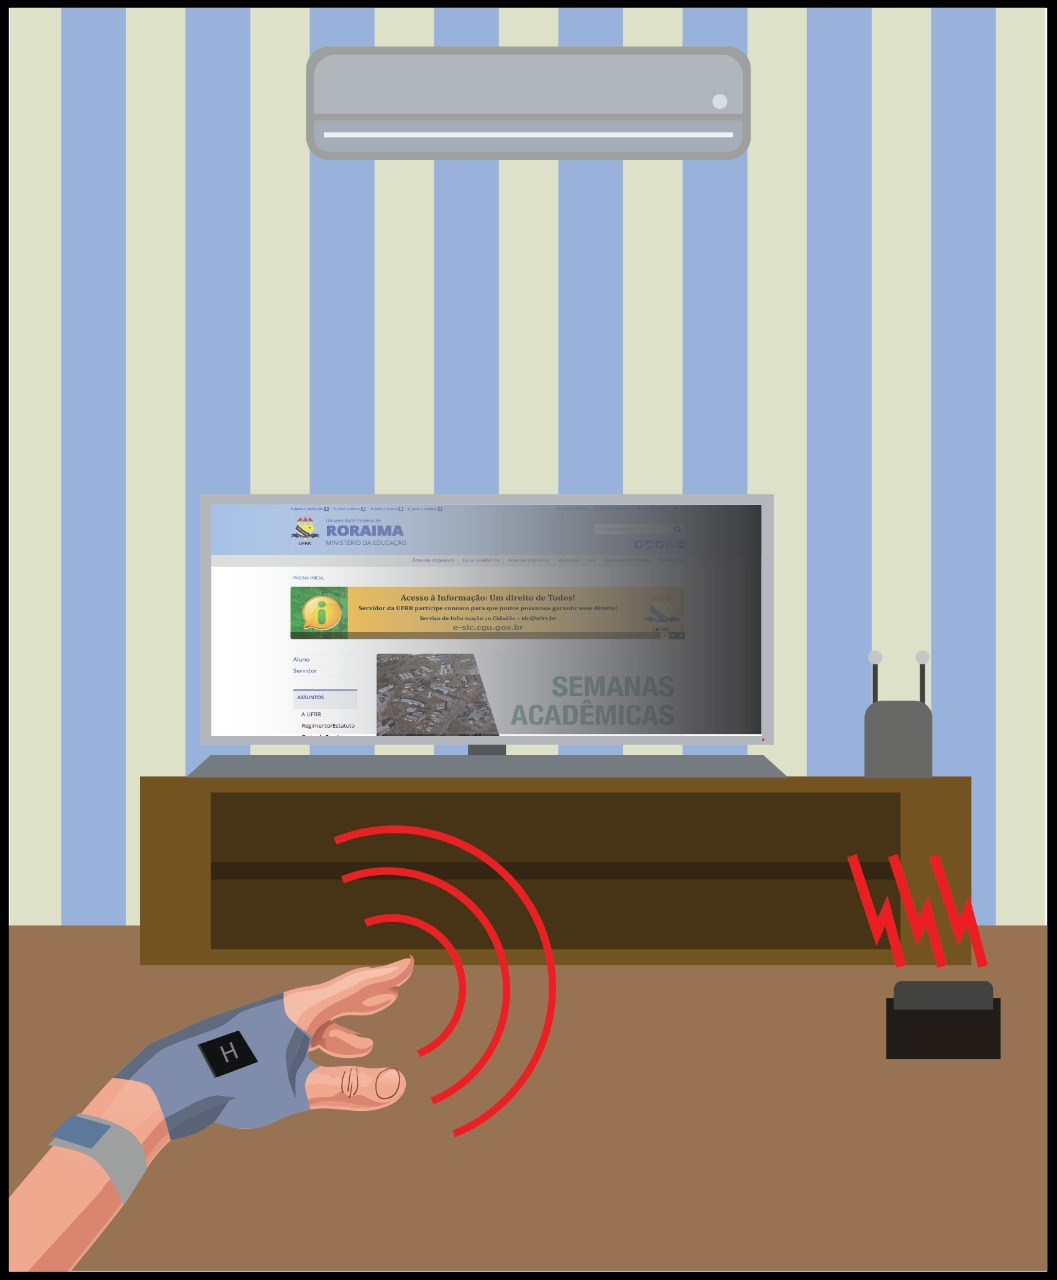
\includegraphics[width=0.5\textwidth, keepaspectratio]{resources/bigpicture.jpeg}
    \caption{Visão geral do protótipo}
    \label{fig:bigpicture}
\end{figure}

Os sinais dos movimentos são processados pela central utilizando algoritmos de aprendizado de máquina, que classificam o gesto realizado e realizam as ações correspondentes que estão definidas no banco de dados do sistema.

%Após os gestos terem sido reconhecidos com sucesso, a central de controle realiza a ação que 

\section{Fluxo de execução da Hand.io}

A~\autoref{fig:fluxograma}, descreve o método proposto para a luva Hand.io através de um fluxograma, mostrando as diferentes etapas de funcionamento da luva de maneira sequencial.

\begin{figure}[ht]
    \centering
	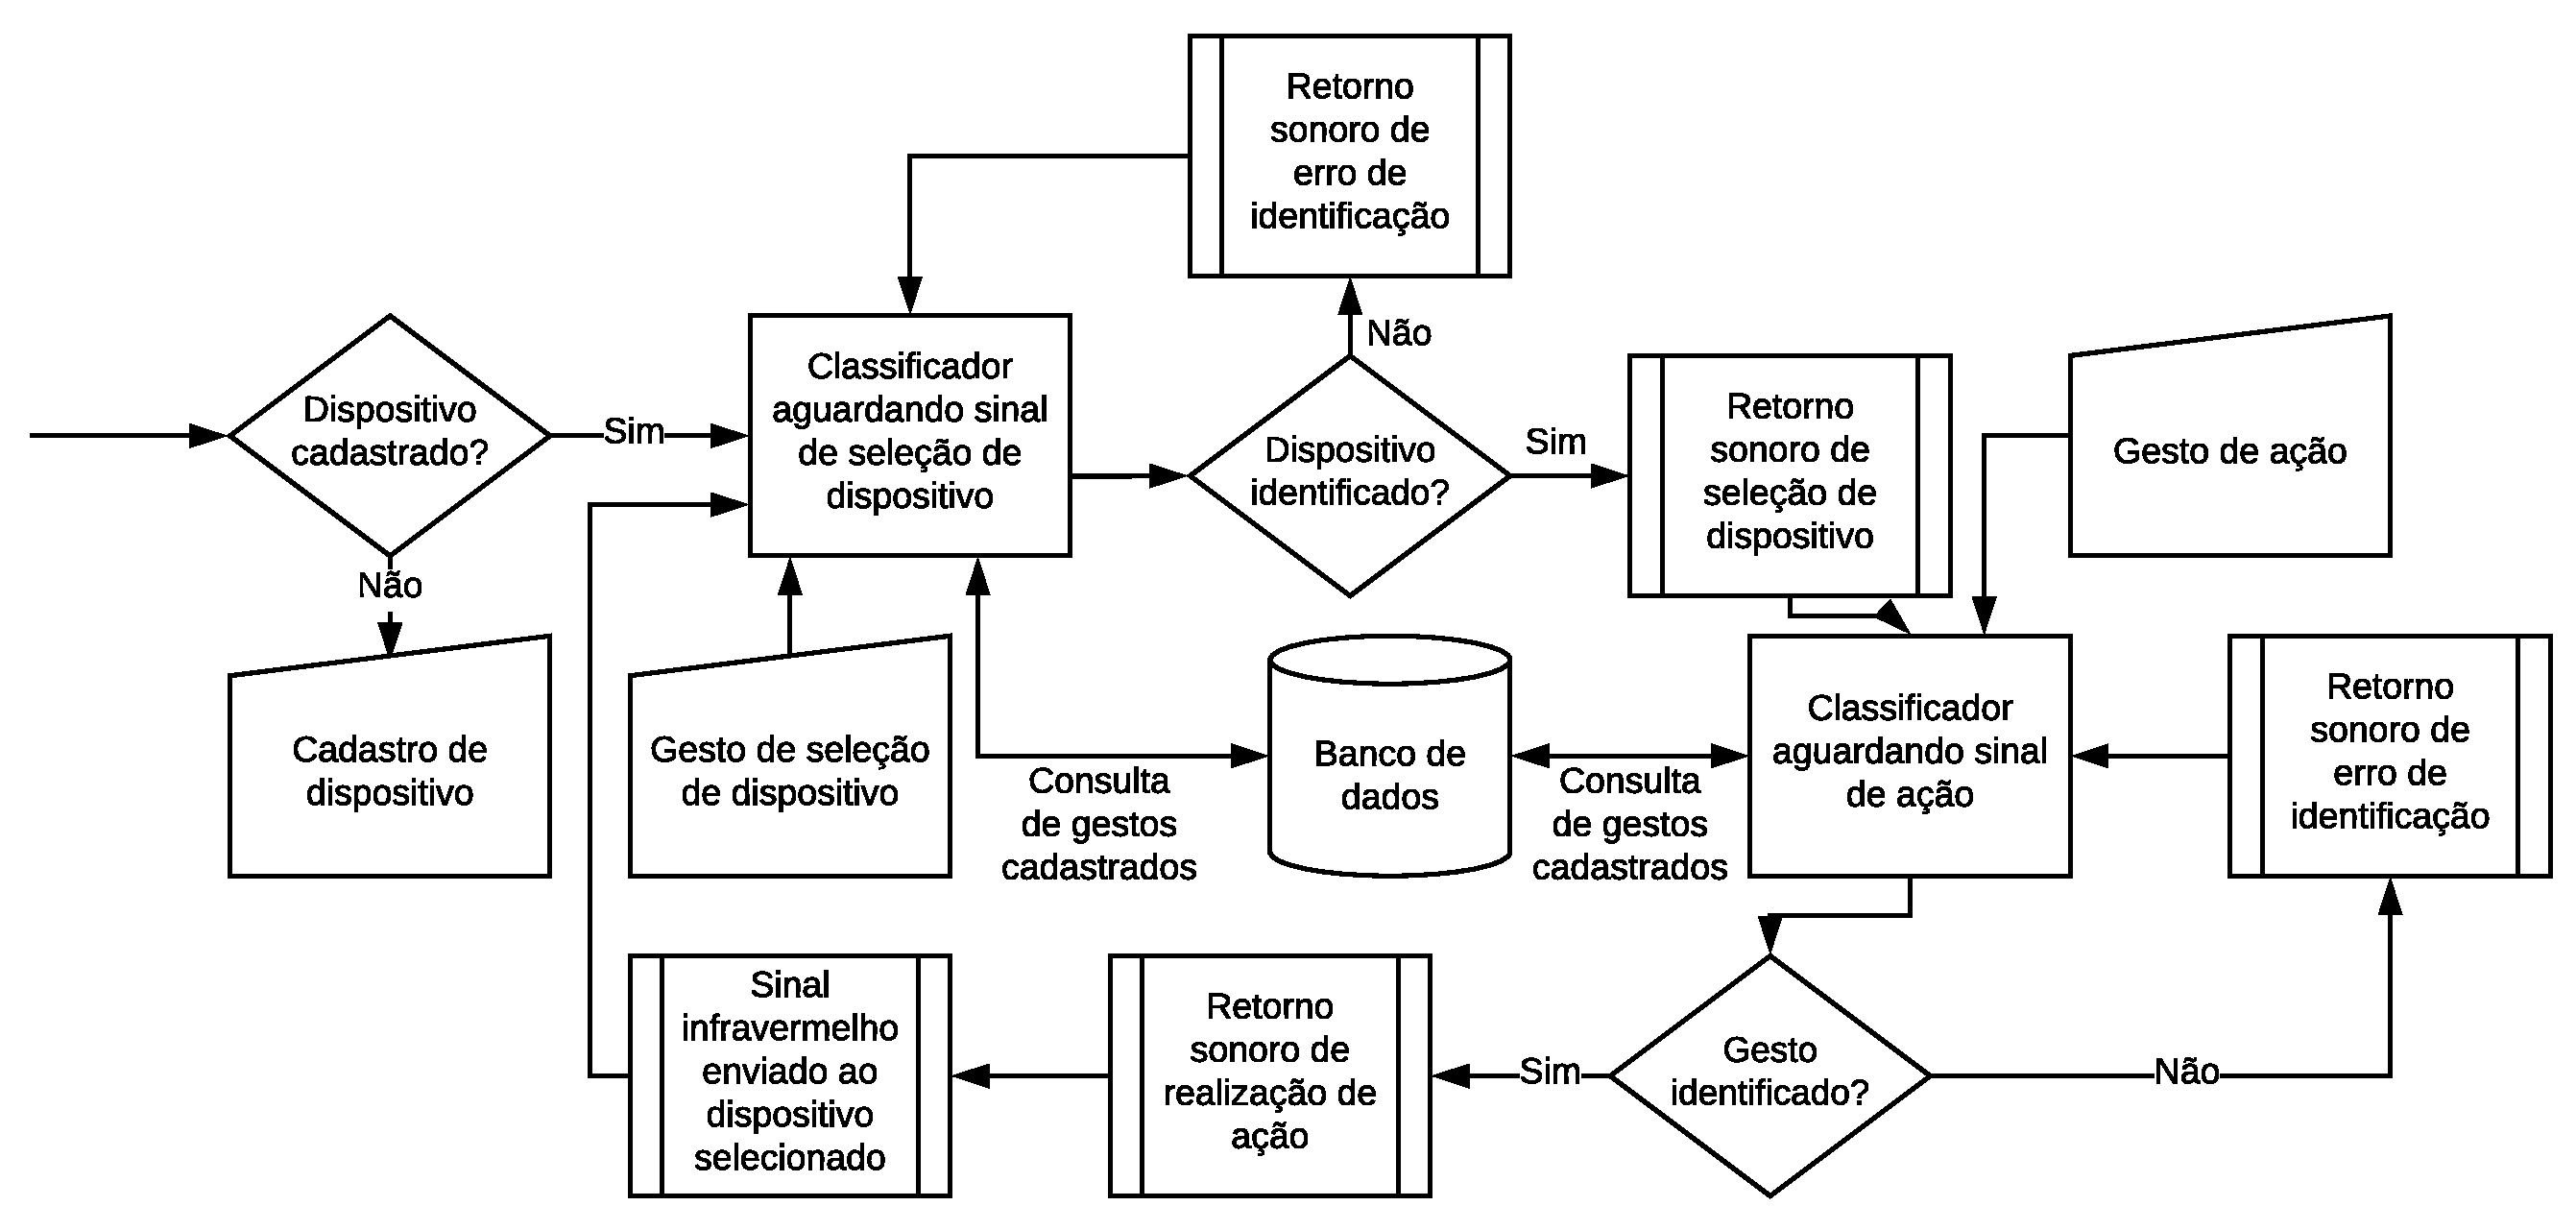
\includegraphics[width=\textwidth, keepaspectratio]{resources/fluxograma.pdf}
	\caption{Fluxograma da Hand.io}
	\label{fig:fluxograma}
\end{figure}

\begin{itemize}
    \item A posição inicial do fluxograma é definida por uma \textbf{seta sem origem} a partir da qual são realizadas as checagens iniciais do sistema.
    \item Os \textbf{losangos} representam condições onde dependendo do resultado o fluxo do sistema pode ser alterado, no primeiro momento é verificada a conexão com a luva de controle e logo depois o sistema verifica se existem dispositivos cadastrados, caso não existam o sistema aguarda pela inserção de dispositivos no banco de dados.
    \item Os \textbf{trapézios} representam ações externas que são realizadas pelo usuário, seja a partir da luva ou a partir do dispositivo que será utilizado para realizar o cadastro de novos dispositivos. 
    \item \textbf{Retângulos} representam processos internos do sistema 
e quadrados com barras laterais representam os processos predefinidos do sistema.
    \item O banco de dados que irá armazenar os dados de gestos e códigos de infra-vermelhos de controle de dispositivos, está representado por um \textbf{cilindro} encontrado na parte central da figura.
\end{itemize}




\section{Captura de Dados Baseado em Movimentos de Amplitude de Punho e Mão}

A ideia principal da luva Hand.io é que o usuário controle seu ambiente utilizando gestos da maneira mais natural possível, para isso os movimentos do usuário são capturados constantemente e enviados para a central em tempo real até que seja identificado um gesto correspondente a um dispositivo cadastrado, como pode ser observado na~\autoref{fig:fluxograma}.

A luva Hand.io utilizará dois sensores para realizar a captura dos movimentos da mão do usuário, um acelerômetro e um giroscópio. Estes dois sensores foram escolhidos visando evitar problemas os encontrados no trabalho de \citeonline{uwave:2009} encontrado na \autoref{cor:uwave} que sofre problemas de precisão devido a presença de apenas um sensor acelerômetro.

Os sensores escolhidos realizam diversas amostras nas mudanças na aceleração e no giro realizados na luva, 



\subsection{Conexão com a central de processamento}

A central de processamento inicia a sua operação esperando o recebimento de algum sinal da luva e até que a conexão tenha sido confirmada, não realiza qualquer ação

A conexão entre a luva e a central será realizada utilizando o protocolo de redes sem fio IEEE 802.11  \cite{802.11:1997}, conhecida popularmente como Wi-Fi, através de uma rede LAN. Os sinais 

\section{Reconhecimento de Padrões Baseado em Movimentos e Ações}

Os sinais recebidos pela central de processamento servem de entrada para algoritmos de aprendizado de máquina que ficam em constante execução tentando classificar os sinais recebidos em categorias previamente escolhidas pelo desenvolvedor do sistema. 

Os possíveis gestos reconhecidos pela luva serão definidos durante a fase de implementação e contarão com a ajuda de um grupo de voluntários que servirão de referência para o desenvolvimento de gestos simples e coesos. O trabalho de \citeonline{imhome:2011} encontrado na \autoref{cor:home} demonstra que um grande volume de gestos personalizados não é pratico do ponto de vista do usuário, pois existe uma quantidade limitada de gestos que podem ser lembrados com precisão sem que haja confusão durante a realização de um determinado gesto.

Será desenvolvido um extensivo \textit{training set} com dados recolhidos de voluntários realizando os gestos. Estes dados serão utilizados como modelo de treinamento para algoritmos de aprendizado de máquina que irão reconhecer os gestos realizados pelo usuário.



Existem dois momentos durante o fluxo de execução da Hand.io onde estes algoritmos são utilizados, quando o sistema aguarda que o usuário selecione o dispositivo que ele deseja controlar e quando o sistema aguarda um comando que será realizado no dispositivo selecionado, ambos os momentos podem ser vistos respectivamente na \autoref{fig:fluxograma} na letra B. A cada vez que os algoritmos finalizam a classificação dos sinais tidos como entrada, o sistema retorna para o usuário um sinal sonoro de confirmação. 




\section{Modelo de Conexão Entre Dispositivos Eletrônicos}

O controle dos dispositivos se dará utilizando um LED infravermelho, seguindo um padrão de controle remoto bem estabelecido pela industria de eletrônicos de consumo. Cada fabricante define códigos infravermelhos específicos para cada dispositivo. Códigos de controle diferentes foram escolhidos visando impedir a interferência entre controles e dispositivos de fabricantes diferentes, como por exemplo o usuário tentar ligar o ar condicionado e acabar ligando a TV por acidente.

Os códigos de controle remoto de cada dispositivo cadastrado no sistema ficarão armazenados em um banco de dados localizado na central de processamento. Cada código estará relacionado à um gesto específico que quando classificado pelo sistema será executado.

%\section{Inferência de Comportamentos para Acionamento de Dispositivos Eletrotônicos}

%Com o passar do uso da luva 

\section{Modelo de Prototipação}

Os componentes utilizados para a confecção do protótipo da luva e da central buscam ter o menor custo possível, sem comprometer a qualidade do sistema. Componentes produzidos em massa que já tem sua utilização testada extensivamente pela comunidade foram selecionados. 

O protótipo é composto pela luva em si que conta com sensores que irão capturar os movimentos do usuário apresentado na \autoref{fig:esq_luva}, e pela central de processamento que irá realizar as ações correspondentes aos gestos exibida na \autoref{fig:esq_central}, nos dispositivos conectados.

A luva será composta por uma placa GY-521 que tem um sensor MPU-6050, apresentado no canto esquerdo da \autoref{fig:esq_luva}. Esta placa é utilizada em diversos projetos que utilizam captura de movimentos devido a sua boa relação custo benefício em relação a precisão dos sensores. O sensor MPU-6050 conta com um acelerômetro de três eixos 



\begin{figure}[ht]
    \centering
    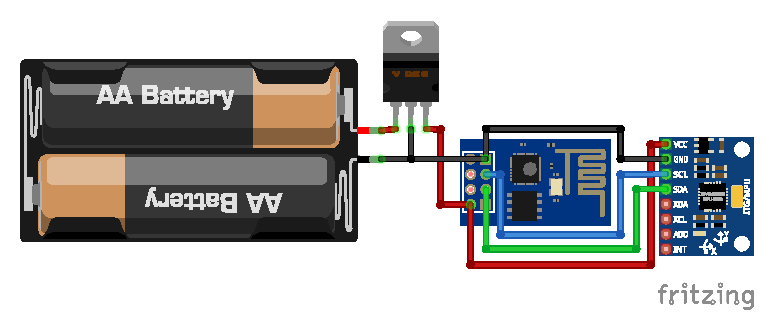
\includegraphics{resources/esquematico_tcc_bb.pdf}
    \caption{Esquemático do protótipo da luva}
    \label{fig:esq_luva}
\end{figure}

\begin{figure}[ht]
    \centering
    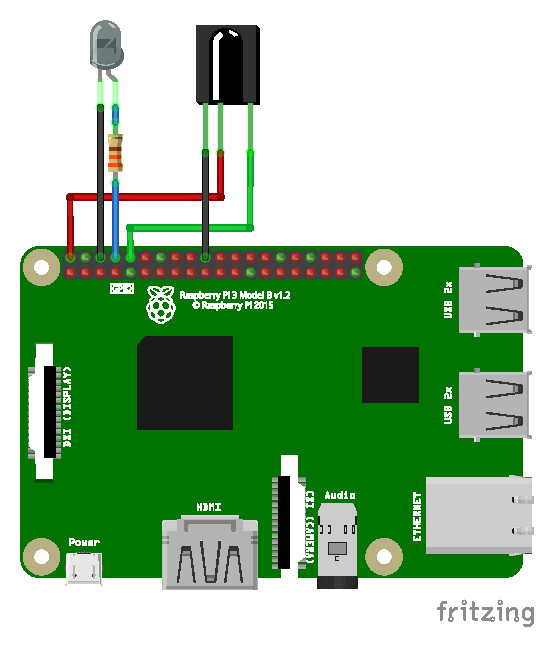
\includegraphics{resources/esquematico_central_bb.pdf}
    \caption{Esquemático da central de processamento de sinais e execução de ações}
    \label{fig:esq_central}
\end{figure}

%\section{Cronograma}